%--------------------------------------------------------------
% thesis.tex 
%--------------------------------------------------------------
% Corso di Laurea in Informatica 
% http://if.dsi.unifi.it/
% @Facolt\`a di Scienze Matematiche, Fisiche e Naturali
% @Universit\`a degli Studi di Firenze
%--------------------------------------------------------------
% - template for the main file of Informatica@Unifi Thesis 
% - based on Classic Thesis Style Copyright (C) 2008 
%   Andr\'e Miede http://www.miede.de   
%--------------------------------------------------------------
\documentclass[openright,twoside,titlepage,fleqn,
	headinclude,12pt,a4paper,BCOR5mm,footinclude,makeidx]{scrbook}
%--------------------------------------------------------------
\usepackage[italian]{babel}
\usepackage[utf8]{inputenc} 
\usepackage[T1]{fontenc} 
\usepackage[square,numbers]{natbib} 
\usepackage[fleqn]{amsmath}  
\usepackage{ellipsis}
\usepackage{listings}
\usepackage{subfig}
\usepackage{caption}
\usepackage{appendix}
\usepackage{siunitx}
\usepackage{lipsum}
%---------------------------------------------------------------
\newcommand{\myItalianTitle}{Titolo italiano\xspace}
\newcommand{\myEnglishTitle}{Titolo inglese\xspace}
\newcommand{\myDegree}{Corso di Laurea Magistrale in Informatica\xspace}
\newcommand{\myCurriculum}{Resilient and secure cyberphysical systems\xspace}
\newcommand{\myName}{Marco Buracchi\xspace}
\newcommand{\myProf}{Michele Boreale\xspace}
\newcommand{\myFaculty}{Scuola di Scienze Matematiche, Fisiche e Naturali\xspace}
\newcommand{\myUni}{\protect{Università degli Studi di Firenze}\xspace}
\newcommand{\myLocation}{Firenze\xspace}
\newcommand{\myTime}{Anno Accademico 2017-2018\xspace}
\newcommand{\myVersion}{Version 0.1\xspace}
\newcommand{\mycopyright}{
\includegraphics[width=1.5cm]{logo/cc.png} 
	\href{https://creativecommons.org/licenses/by-nc-sa/4.0/}{Creative
		Commons Attribution-NonCommercial-ShareAlike 4.0 International (CC BY-NC-SA 4.0)  }\xspace}
%--------------------------------------------------------------

\newcommand{\disps}{dispositivo crittografico }
\newcommand{\dispp}{dispositivi crittografici }

%--------------------------------------------------------------
\usepackage{dia-classicthesis-ldpkg}
%--------------------------------------------------------------
% Options for classicthesis.sty:
% tocaligned eulerchapternumbers drafting linedheaders 
% listsseparated subfig nochapters beramono eulermath parts 
% minionpro pdfspacing
\usepackage[eulerchapternumbers,linedheaders,subfig,beramono,eulermath,
parts,dottedtoc]{classicthesis}
%--------------------------------------------------------------
\newlength{\abcd} % for ab..z string length calculation
% how all the floats will be aligned
\newcommand{\myfloatalign}{\centering} 
\setlength{\extrarowheight}{3pt} % increase table row height
\captionsetup{format=hang,font=small}
%--------------------------------------------------------------
% Layout setting
%--------------------------------------------------------------
\graphicspath{{img/}}
\usepackage{geometry}
\geometry{
	a4paper,
	ignoremp,
	bindingoffset = 1cm, 
	textwidth     = 13.5cm,
	textheight    = 21.5cm,
	lmargin       = 3.5cm, % left margin
	tmargin       = 4cm    % top margin 
}

\lstset{
  	frame=tb,
	language=Matlab,
  	aboveskip=3mm,
  	belowskip=3mm,
  	showstringspaces=false,
  	columns=flexible,
  	basicstyle={\small\ttfamily},
  	numbers=none,
  	breaklines=true,
  	breakatwhitespace=true,
  	tabsize=3
}
\usepackage[italian,noabbrev]{cleveref}
\usepackage{imakeidx}
\makeindex[intoc]
%--------------------------------------------------------------
\begin{document}
\frenchspacing
\raggedbottom
\pagenumbering{roman}
\pagestyle{plain}
%--------------------------------------------------------------
% Frontmatter
%--------------------------------------------------------------
%--------------------------------------------------------------
% titlepage.tex (use thesis.tex as main file)
%--------------------------------------------------------------
\begin{titlepage}
	\begin{center}
   	\large
      \hfill
      \vfill
      \begingroup
         
\includegraphics[scale=0.15]{logo/LOGO}\\
%			\spacedallcaps{\myUni} \\ 
			\myFaculty \\
			\vspace{0.5cm}
			\myDegree \\ 
			Curriculum: \emph{\myCurriculum}\\
			\vspace{0.5cm}
         \vspace{0.5cm}    
         Tesi di Laurea Magistrale 
      \endgroup 
      \vfill 
      \begingroup
      	\color{Maroon}\spacedallcaps{\myItalianTitle} \\ $\ $\\
      	\spacedallcaps{\myEnglishTitle} \\ 	
	\bigskip
      \endgroup
      \spacedlowsmallcaps{\myName}
      \vfill 
      \vfill
      Relatore: Prof. \emph{\myProf}\\
      \vfill
      \vfill
      \myTime
      \vfill                      
	\end{center}        
\end{titlepage}   
%--------------------------------------------------------------
% back titlepage
%--------------------------------------------------------------
   \newpage
	\thispagestyle{empty}
	\hfill
	\vfill
	\noindent\myName: 
	\textit{\myItalianTitle,} 
	\myDegree, \mycopyright, \myUni, \myTime
%--------------------------------------------------------------
% back titlepage end
%--------------------------------------------------------------
\pagestyle{scrheadings}
%--------------------------------------------------------------
% Mainmatter
%--------------------------------------------------------------
\pagenumbering{arabic}
% use \cleardoublepage here to avoid problems with pdfbookmark
%\chapter{Introduzione}
	prova \cite{kocher2018spectre}.
 % use \myChapter command instead of \chapter
%\cleardoublepage\myPart{Part I}
%\include{chapter01}
%\cleardoublepage\myPart{Part II}
%\include{chapter02}
%\include{chapter03}
\tableofcontents
\listoffigures
\listoftables
\cleardoublepage
\thispagestyle{empty}
\begin{flushright}
\null\vspace{\stretch {1}}
\emph{"Da campo a campo, nel tetro grembo della notte,\\s’avverte appena il brusio di entrambe le armate,\\sicché le sentinelle appostate quasi possono udire\\i mormorii furtivi delle sentinelle nemiche" \break --- Enrico V, William Shakespear} \vspace{\stretch{2}}\null
\end{flushright}
\cleardoublepage
%----------------CAPITOLI--------------------------------------
\chapter{Introduzione}
	prova \cite{kocher2018spectre}.

\chapter{Side-channel attacks}

	I \emph{side-channel attacks} sono metodi di criptanalisi che sfruttano le side-channels informations insieme ad altre tecniche di analisi per recuperare la chiave utilizzata da un \disps\cite{standaert2010introduction}.\begin{figure}
		
		\begin{center}
			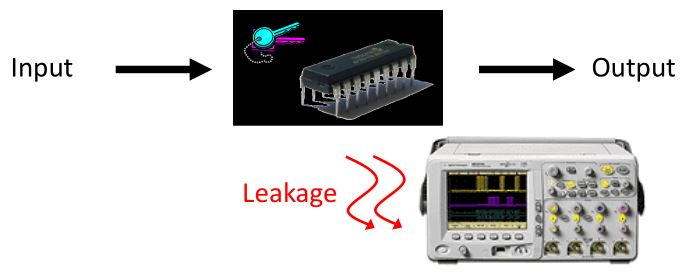
\includegraphics[scale=.6]{sideChannelLeakage}
			\caption{Esempio di side-channel attack}
			\label{fig:attack}
		\end{center}
	\end{figure}
	
	Nella \cref{fig:attack} si può vedere una configurazione tipo di side-channel attack. Da una parte c'è il dispositivo che implementa la funzione crittografica e accanto c'è lo strumento utilizzato per rilevare le grandezze fisiche prodotte dal dispositivo attaccato. La cosa fondamentale è che questo tipo di attacchi non vanno a colpire direttamente la funzione crittografica ma sfruttano le informazioni fisiche dell'ambiente intorno al dispositivo.
	
	L'analisi di questi metodi ha acquisito notevole interesse dato che questo tipo di attacchi possono essere montati velocemente e molto spesso non richiedono hardware particolare e costoso. Con pochi euro si possono ad esempio acquistare in comuni negozi di bricolage o elettronica apparecchi in grado di analizzare il consumo elettrico di un dispositivo. Con tali apparecchi è possibile montare in pochi secondi un attacco di tipo \emph{Simple Power Analysis}\cite{mangard2002simple} che verrà spiegato più avanti. 
	
	Il governo degli USA, nel suo "Orange book"\cite{latham1986department} indica dei requisiti di sicurezza per i sistemi operativi. Questo documento introduce i primi standard per l'\emph{information leakage}. Purtroppo la letteratura specializzata è però molto variegata e disomogenea quindi, come prima cosa, cerchiamo di trovare un modo per classificare i vari tipi di attacchi in maniera tale da avere una visione più sistemistica del settore.
	
	\section{Background}
	
		In questa sezione verranno stabiliti dei parametri per classificare i vari tipi di attacchi side-channel.
	
		\subsection{Tipi di canali}
	
			Nel lavoro di \emph{Ge, Yarom, Cock e Heiser}\cite{ge2016survey} vengono fornite alcune definizioni che utilizzeremo nel prosieguo di questa tesi. La prima distinzione che è necessario fare è quella tra side-channel e \emph{covert-channel}. Con i primi ci si riferisce ai canali che lasciano \emph{accidentalmente} filtrare informazioni sensibili (ad esempio una chiave crittografica) in una comunicazione tra due partecipanti fidati. I secondi sono quelli creati e sfruttati dall'attaccante ad esempio tramite l'utilizzo di Trojan e che \emph{deliberatamente} lasciano filtrare le informazioni. In questo lavoro verranno trattati solamente i primi.
			
			L'altra differenza fondamentale per quello che riguarda i canali è quella tra canali di tipo \emph{storage} e canali di tipo \emph{timing}. I canali di tipo storage vengono sfruttati per ottenere qualcosa di direttamente visibile nel sistema (valore dei registri, valore di ritorno di una system call, ecc.). Quelli di tipo timing vengono sfruttati andando ad osservare variazioni del tempo di esecuzione di un programma (o di parti di esso).
			
		\subsection{Tipi di attacco}
		
			\emph{Standaert} nel suo lavoro \cite{standaert2010introduction} utilizza altre due dimensioni interessanti per classificare questi attacchi; l'\emph{invasività} e l'\emph{attività}. 
			
			Si definisce invasivo un attacco che richiede un disassemblamento del dispositivo attaccato per avere accesso diretto ai suoi componenti interni (wiretapping o sensori collegati direttamente all'hardware). Un attacco non invasivo, al contrario, sfrutta solamente le informazioni disponibili esternamente (quasi sempre involontarie) come il tempo d'esecuzione o l'energia consumata.
			
			Si definisce attivo un attacco che cerca di interferire con il corretto funzionamento del dispositivo (fault-injection) mentre un attacco passivo si limita ad osservare il comportamento del dispositivo durante il suo lavoro senza disturbarlo. 
			
		\subsection{Grandezza fisica osservata}
		
			Una caratteristica principale di questi attacchi è sicuramente la grandezza fisica che viene osservata per montare l'attacco. Teoricamente, qualunque grandezza fisica misurabile può essere sfruttata ma alcune si prestano maggiormente rispetto ad altre. 
			
			Il tempo e il consumo energetico sono le più sfruttate ma non sono di certo le uniche. \emph{Genkin, Shamir e Tromer} nel loro lavoro \cite{genkin2014rsa} vanno ad ascoltare i rumori prodotti dal processore. \emph{Ferrigno e Hlavac}\cite{ferrigno2008aes} osservano la luce (qualche fotone) emessa dai transistor nel passaggio di stato da 0 a 1. \emph{Martinasek, Zeman e Trasy} sfruttano i campi elettromagnetici creati dai chip. \emph{Giraud}\cite{giraud2004dfa} sfrutta la tecnica della fault-injection e analizza i risultati delle computazioni.
			
			Questo elenco assolutamente non esaustivo delle tecniche utilizzate può far capire quanto variegato ed eterogeneo (nonché in continua evoluzione) sia questo settore.
			
			Tutti questi attacchi (e anche altri) verranno approfonditi più avanti.
			
		\subsection{Hardware attaccato}
		
			Gli attacchi possono essere suddivisi anche in base alla componente hardware che viene attaccata. Anche in questo caso ci sono componenti più attaccati di altri (cache e processori) ma non mancano esempi di attacchi a monitor\cite{van1985electromagnetic}, tastiere\cite{asonov2004keyboard} o stampanti\cite{backes2010acoustic}.
			
		\subsection{Algoritmo attaccato}
		
			Un'ultima classificazione può essere effettuata andando a discriminare gli attacchi secondo l'algoritmo crittografico attaccato. In questo caso i due maggiori algoritmi attaccati sono senza dubbio AES ed RSA.
			
			\begin{table}[]
				\centering
				\caption{Classificazione dei principali attacchi analizzati}
				\label{tab:attacchi}
				\begin{tabular}{c|c|c|c|c|c} \hline
					Articolo 					& Grandezza                    & Hardware   & Algoritmo & Invasivo & Attivo \\ \hline
					\cite{genkin2014rsa}		& Suono                        & CPU        & RSA       & No       & No     \\ \hline
					\cite{ferrigno2008aes}		& Luce                         & Transistor & AES       & Sì       & No     \\ \hline
					\cite{kocher2018spectre}	& Tempo                        & Cache      & RSA       & No       & No     \\ \hline
					\cite{mangard2002simple}	& Consumo elettrico            & Smartcard  & AES       & No       & No     \\ \hline
					\cite{martinasek2012simple}	& Campo elettromagnetico       & Chip       & AES       & No       & No     \\ \hline
					\cite{giraud2004dfa}		& Risultato della computazione & Smartcard  & AES       & Sì       & Sì    
				\end{tabular}
			\end{table}
		
			Nella \cref{tab:attacchi} si è provato a classificare con i criteri sopra definiti i 6 attacchi che verranno approfonditi in questo lavoro.
			
	\section{Attacchi basati sul suono}
	\lipsum[1-5]
	\section{Attacchi basati sulla luce}
	\lipsum[1-5]
	\section{Attacchi basati sul tempo}
	\lipsum[1-5]
	\section{Attacchi basati sul consumo elettrico}
	\lipsum[1-5]
	\section{Attacchi basati sul campo elettromagnetico}
	\lipsum[1-5]
	\section{Attacchi basati sui risultati delle computazioni}
	\lipsum[1-5]
\chapter{Cache attacks}
\lipsum
\chapter{SPECTRE attacks}
\lipsum
\chapter{Quantitative Information-flow Analysis}
\lipsum
%-----------------BIBLIOGRAFIA---------------------------------
\bibliography{bib/bibliografia}
\bibliographystyle{unsrt}
%--------------------------------------------------------------
\addcontentsline{toc}{chapter}{Acronimi}
\chapter*{Acronimi}
\begin{acronym}[CAGD]
	\acro{AES}{Advanced Encryption Standard}
	\acro{CNES}{Centre National d’Etudes Spatiales}
	\acro{DES}{Data Encryption Standard}
	\acro{DPA}{Differential Power Analysis}
	\acro{HTTPS}{HyperText Transfer Protocol over Secure Socket Layer}
	\acro{LED}{Light Emitting Diode}
	\acro{PICA}{Picosecond Imaging Circuit Analysis}
	\acro{SPA}{Simple Power Analysis}
  	\acro{USB}{Universal Serial Bus}
\end{acronym}
\printindex
\end{document}
%--------------------------------------------------------------
